\newcommand\user[2]{
	\begin{scope}[xshift=#1cm, yshift=#2cm]
		\clip (0, 0) circle (0.5);
		\fill[black] (0, 0) circle (0.5);
		\fill[white] (0, 0) circle (0.48);
		\fill[black] (0, -0.675) circle (0.4);
		\fill[black] (0, 0.075) circle (0.24);
  \end{scope}
}

\newcommand\ip[2]{
	\begin{scope}[xshift=#1cm, yshift=#2cm]
		%\rectangle[fill=black, rounded corners=0.2cm] (-0.5, -0.7) -- (0.5, 0.7);
		\draw[fill=black, thick, rounded corners=0.15cm] (-0.3, -0.5) rectangle (0.3, 0.5);
		\draw[fill=white] (0, -0.3) circle (0.1);
		\draw[fill=white, rounded corners=0.07cm] (-0.2, -0.1) rectangle (0.2, 0.0);
		\draw[fill=white, rounded corners=0.07cm] (-0.2, 0.1) rectangle (0.2, 0.2);
		\draw[fill=white, rounded corners=0.07cm] (-0.2, 0.3) rectangle (0.2, 0.4);
  \end{scope}
}

\newcommand\www[2]{
	\begin{scope}[xshift=#1cm, yshift=#2cm]
		\clip (0, 0) circle (0.5);
		\fill[yellow!65!black] (0, 0) circle (0.5);
		\fill[white] (-0.5, -0.175) rectangle (0.5,0.175);
		\node[text=yellow!65!black] at (0,0) {www};
  \end{scope}
}

\newcommand\malwww[2]{
	\begin{scope}[xshift=#1cm, yshift=#2cm]
		\clip (0, 0) circle (0.5);
		\fill[red!65!black] (0, 0) circle (0.5);
		\fill[white] (-0.5, -0.175) rectangle (0.5,0.175);
		\node[text=yellow!65!black] at (0,0) {www};
  \end{scope}
}

\newcommand\wwwline[3]{
	\node[circle, minimum size=1.1cm] (#3) at (0, #1) {};
	\www{0}{#1}
	\node[text width=50mm, align=right] at (-3.5, #1) {#2};
}

\newcommand\malwwwline[3]{
	\node[circle, minimum size=1.1cm] (#3) at (0, #1) {};
	\malwww{0}{#1}
	\node[text width=50mm, align=right] at (-3.5, #1) {#2};
}

\newcommand\userline[2]{
	\node[circle, minimum size=1.1cm] (#2) at (5, #1) {};
	\user{5}{#1}
	\node[text width=50mm, align=left] at (8.5, #1) {#2};
}

\newcommand\ipline[3]{
	\node[circle, minimum size=1.1cm] (#3) at (5, #1) {};
	\ip{5}{#1}
	\node[text width=50mm, align=left] at (8.5, #1) {#2};
}

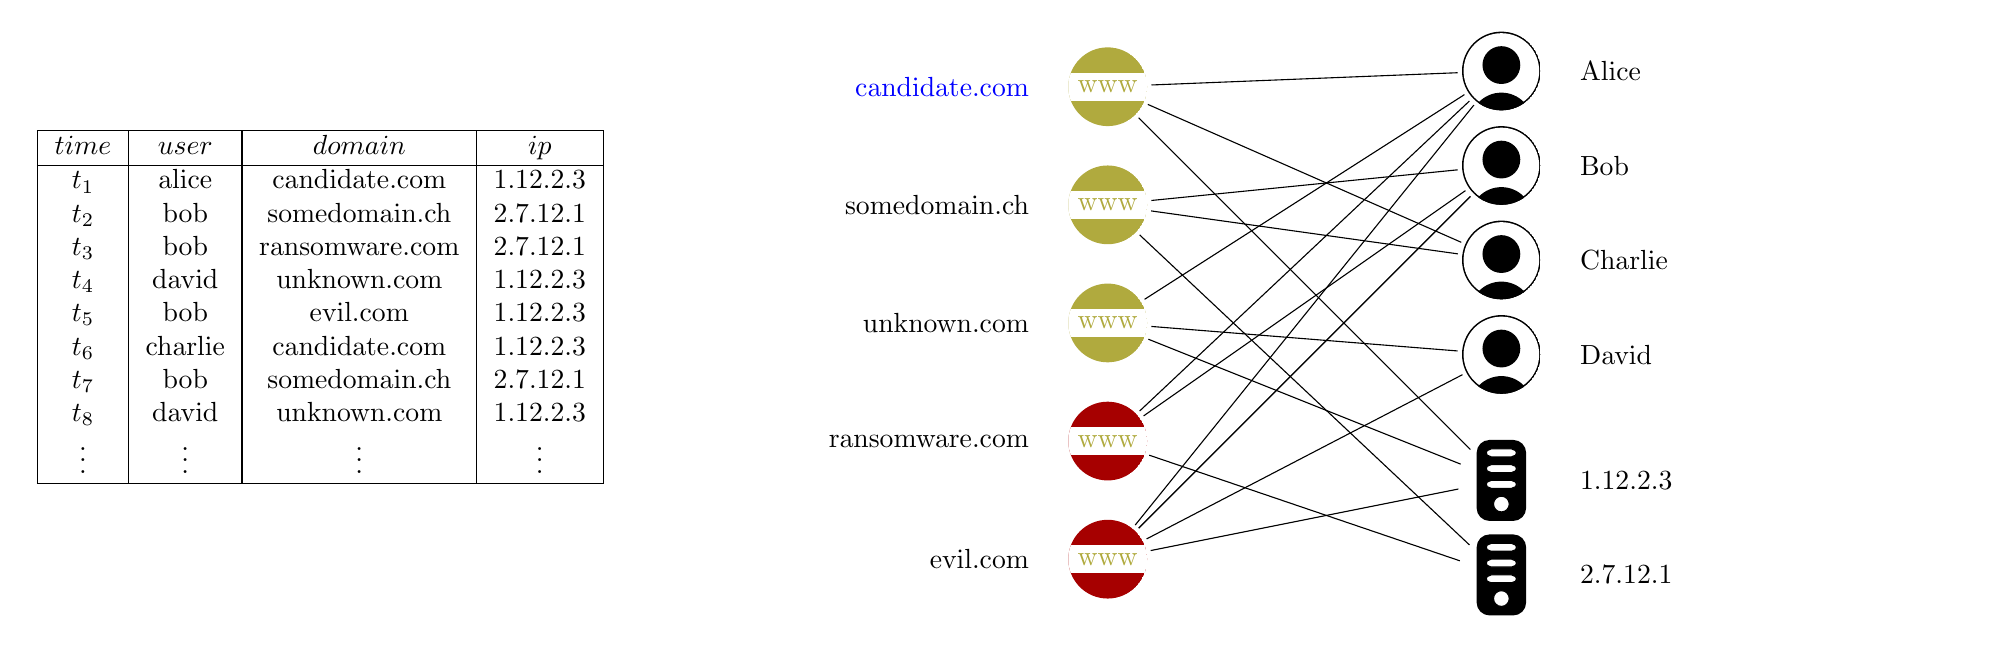
\begin{tikzpicture}
\uncover<2->{
\node at (-10, 1.2) (x)
{
\begin{tabular}{|c|c|c|c|}
\hline
$\bm{time}$ & $\bm{user}$ & $\bm{domain}$ & $\bm{ip}$ \\
\hline
$t_1$&alice& candidate.com& 1.12.2.3\\
$t_2$&bob& somedomain.ch& 2.7.12.1\\
$t_3$&bob& ransomware.com& 2.7.12.1\\
$t_4$&david& unknown.com & 1.12.2.3\\
$t_5$&bob& evil.com & 1.12.2.3 \\
$t_6$&charlie& candidate.com & 1.12.2.3 \\
$t_7$&bob & somedomain.ch& 2.7.12.1 \\
$t_8$&david& unknown.com & 1.12.2.3\\
\vdots &\vdots &\vdots &\vdots \\
\hline
\end{tabular}
};
}
%{
%$\left\{\begin{array}{c}
%alice, candidate.com, 1.12.2.3\\
%bob, somedomain.ch, 2.7.12.1\\
%bob, ransomware.com, 2.7.12.1\\
%david, unknown.com , 1.12.2.3\\
%bob, evil.com , 1.12.2.3 \\
%charlie, candidate.com , 1.12.2.3 \\
%bob, somedomain.ch, 2.7.12.1 \\
%\dots
%\end{array}\right\}$};
%}
\uncover<3->{
	\malwwwline{-2}{evil.com}{D1};
	\malwwwline{-0.5}{ransomware.com}{D2};
	\wwwline{4}{\textcolor{blue}{candidate.com}}{D5};
	\ipline{-1}{1.12.2.3}{i1}
	\userline{4.2}{Alice};
	\draw (Alice) -- (D1);
  \draw (Alice) -- (D2);
  \draw (i1) -- (D1);
  \draw (Alice) -- (D5);
	\draw (i1) -- (D5);
	\wwwline{1}{unknown.com}{D3};
	\wwwline{2.5}{somedomain.ch}{D4};
	\ipline{-2.2}{2.7.12.1}{i2}
	\userline{0.6}{David};
	\userline{1.8}{Charlie};
	\userline{3}{Bob};
  \draw (Alice) -- (D3);
  \draw (Bob) -- (D1);
  \draw (Bob) -- (D2);
  \draw (Bob) -- (D1);
  \draw (David) -- (D1);
  \draw (i2) -- (D2);
  \draw (Bob) -- (D4);
  \draw (David) -- (D3);
  \draw (Charlie) -- (D4);
  \draw (Charlie) -- (D5);
  \draw (i1) -- (D3);
  \draw (i2) -- (D4);

}
\end{tikzpicture}
